% das Paket "flashcards" erzeugt Karteikarten zum lernen
% auf der Vorderseite steht das Buzzword oder die Frage
% auf der Rückseite steht die Antwort
% beim ausdrucken auf doppelseitiges Drucken achten
%
\documentclass[avery5371]{flashcards}
\usepackage[utf8]{inputenc}
\usepackage[]{amsmath} 
\usepackage[]{amssymb}
\usepackage{bussproofs} % prooftrees
\usepackage{mdwlist} % less space for lists
\cardfrontstyle{headings}
\begin{document}
%%%%%%%%%%%%%%%%%%%%%%%%%%%%%%%%%%%%%

\begin{flashcard}[Natürliches Schließen ]{ 4 Probleme natürlicher Sprache }
    \begin{enumerate*}
        \item Zuordnung von Wahrheitswerten zu Aussagen ist problematisch.
        \item Natürliche Sprache ist oft schwer verständlich.
        \item Natürliche Sprache ist mehrdeutig.
        \item Natürliche Sprache hängt von Kontext ab.
    \end{enumerate*}
\end{flashcard}

\begin{flashcard}[Natürliches Schließen ]{ was sind Formeln? }
    \begin{enumerate*}
        \item Alle atomaren Formeln und $\bot$ sind Formeln.
        \item Falls $\varphi$ und $\psi$ Formeln sind, sind auch $(\varphi\wedge\psi),(\varphi\wedge\psi)$($\varphi \rightarrow\psi$)und $\lnot\varphi$Formeln.
        \item Nichts ist Formel, was sich nicht mittels der obigen Regeln erzeugen läßt.
    \end{enumerate*}
\end{flashcard}

\begin{flashcard}[Natürliches Schließen ]{ Bezeichnungen in Formeln }
    \begin{itemize*}
        \item Falsum: $\bot$
        \item Konjunktion: $\wedge$
        \item Disjunktion: $\vee$
        \item Implikation: $\rightarrow$
        \item Negation: $\lnot$
    \end{itemize*}
\end{flashcard}

\begin{flashcard}[ Natürliches Schließen ]{ $(\bigvee_{i=1}^n \varphi_i)$ statt ... }
    $(\bigvee_{i=1}^n \varphi_i$ statt $(...((\varphi_1\vee\varphi_2)\vee\varphi_3)\vee...\vee\varphi_n)$
\end{flashcard}

\begin{flashcard}[ Natürliches Schließen ]{ $(\bigwedge_{i=1}^n \varphi_i)$ statt ... }
    $(\bigwedge_{i=1}^n \varphi_i)$ statt $(...((\varphi_1\wedge\varphi_2)\wedge\varphi_3)\wedge...\wedge\varphi_n)$
\end{flashcard}

\begin{flashcard}[ Natürliches Schließen ]{ $(\varphi \leftrightarrow \psi)$ statt ... }
    $(\varphi \leftrightarrow \psi)$ statt $((\varphi\rightarrow\psi)\wedge(\psi\rightarrow\varphi))$
\end{flashcard}

\begin{flashcard}[ Natürliches Schließen ]{ Präzedenz der Operatoren }
    \begin{itemize*}
        \item $\leftrightarrow$ bindet am schwächsten
        \item $\rightarrow$...
        \item $\vee$...
        \item $\wedge$...
        \item $\lnot$ bindet am stärksten
    \end{itemize*}
\end{flashcard}

\begin{flashcard}[ Natürliches Schließen ]{ triviale Deduktion }
    Aus der Annahme der Aussage $\varphi$ folgt $\varphi$ unmittelbar.

    $\varphi$ mit Hypothesen $\{\varphi\}$ und Konklusion $\varphi$.
\end{flashcard}

\begin{flashcard}[ Natürliches Schließen ]{ Konjunktionseinführung }
    Ist D eine Deduktion von $\varphi$ mit Hypothesen aus $\Gamma$ und ist E eine Deduktion von $\psi$ mit Hypothesen aus $\Gamma$, so ergibt sich die folgende Deduktion von $\varphi\wedge\psi$ mit Hypothesen aus $\Gamma$:

    \begin{prooftree}
        \AxiomC{$\varphi$}
        \AxiomC{$\psi$}
        \RightLabel{\scriptsize ($\wedge I$)}
        \BinaryInfC{$\varphi\wedge\psi$}
    \end{prooftree}
    %\includegraphics[width=.5\linewidth]{Assets/Logik-konjunktionseinführung.png}
\end{flashcard}

\begin{flashcard}[ Natürliches Schließen ]{ Konjunktionselimination }
    Ist D eine Deduktion von $\varphi\wedge\psi$ mit Hypothesen aus $\Gamma$, so ergeben sich die folgenden Deduktionen von $\varphi$ bzw. von $\psi$ mit Hypothesen aus $\Gamma$:

    \begin{prooftree}
        \AxiomC{$\varphi\wedge\psi$}
        \RightLabel{\scriptsize ($\wedge E_1$)}
        \UnaryInfC{$\varphi$}
    \end{prooftree}

    \begin{prooftree}
        \AxiomC{$\varphi\wedge\psi$}
        \RightLabel{\scriptsize ($\wedge E_2$)}
        \UnaryInfC{$\psi$}
    \end{prooftree}
    %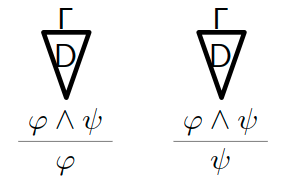
\includegraphics[width=.5\linewidth]{Assets/Logik-Konjunktionselimination.png}
\end{flashcard}

\begin{flashcard}[ Natürliches Schließen ]{ Implikationseinführung }
    Ist D eine Deduktion von $\psi$ mit Hypothesen aus $\Gamma\cup\{\varphi\}$, so ergibt sich die folgende Deduktion von $\varphi\rightarrow\psi$ mit Hypothesen aus $\Gamma$:

    \begin{prooftree}
        \AxiomC{[$\varphi$]}\noLine
        \UnaryInfC{$\psi$}
        \RightLabel{\scriptsize ($\rightarrow I$)}
        \UnaryInfC{$\varphi\rightarrow\psi$}
    \end{prooftree}
    %\includegraphics[width=.5\linewidth]{Assets/Logik-Implikationseinführung.png}
\end{flashcard}

\begin{flashcard}[ Natürliches Schließen ]{ Implikationselimination }
    oder modus ponens

    Ist D eine Deduktion von $\varphi$ mit Hypothesen aus $\Gamma$ und ist E eine Deduktion von $\varphi\rightarrow\psi$ mit Hypothesen aus $\Gamma$, so ergibt sich die folgende Deduktion von $\psi$ mit Hypothesen aus $\Gamma$:

    \begin{prooftree}
        \AxiomC{$\varphi$}
        \AxiomC{$\varphi\rightarrow\psi$}
        \RightLabel{\scriptsize ($\rightarrow E$)}
        \BinaryInfC{$\psi$}
    \end{prooftree}
    %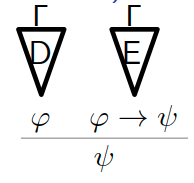
\includegraphics[width=.5\linewidth]{Assets/Logik-Implikationselimination.png}
\end{flashcard}

\begin{flashcard}[ Natürliches Schließen ]{ Disjunktionselimination }
    oder Fallunterscheidung

    Ist D eine Deduktion von $\varphi\vee\psi$ mit Hypothesen aus $\Gamma$, ist E eine Deduktion von $\sigma$ mit Hypothesen aus $\Gamma\cup\{\varphi\}$und ist F eine Deduktion von $\sigma$ mit Hypothesen aus $\Gamma\cup\{\psi\}$, so ergibt sich die folgende Deduktion von $\sigma$ mit Hypothesen aus $\Gamma$:

    \begin{prooftree}
        \AxiomC{$\varphi\vee\psi$}
        \AxiomC{[$\varphi$]}\noLine
        \UnaryInfC{$\delta$}
        \AxiomC{[$\psi$]}\noLine
        \UnaryInfC{$\delta$}
        \RightLabel{\scriptsize ($\vee E$)}
        \TrinaryInfC{$\psi$}
    \end{prooftree}
    %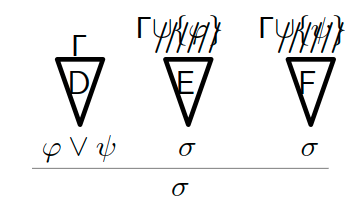
\includegraphics[width=.5\linewidth]{Assets/Logik-Disjunktionselimination.png}
\end{flashcard}

\begin{flashcard}[ Natürliches Schließen ]{ Disjunktionseinführung }
    \begin{prooftree}
        \AxiomC{$\varphi$}
        \RightLabel{\scriptsize ($\vee I_1$)}
        \UnaryInfC{$\varphi\vee\psi$}
    \end{prooftree}

    \begin{prooftree}
        \AxiomC{$\psi$}
        \RightLabel{\scriptsize ($\vee I_2$)}
        \UnaryInfC{$\varphi\vee\psi$}
    \end{prooftree}
    %$$\frac{\varphi}{\varphi\vee\psi} (\vee I_1) \quad \frac{\psi}{\varphi\vee\psi} (\vee I_2)$$
\end{flashcard}

\begin{flashcard}[ Natürliches Schließen ]{ Negationseinführung }
    Ist D eine Deduktion von $\bot$ mit Hypothesen aus $\Gamma\cup\{\varphi\}$, so ergibt sich die folgende Deduktion von $\lnot\varphi$ mit Hypothesen aus $\Gamma$:
    \begin{prooftree}
        \AxiomC{[$\varphi$]}\noLine
        \UnaryInfC{$\bot$}
        \RightLabel{\scriptsize ($\lnot I$)}
        \UnaryInfC{$\lnot\varphi$}
    \end{prooftree}
    %\includegraphics[width=.5\linewidth]{Assets/Logik-Negationseinführung.png}
\end{flashcard}

\begin{flashcard}[ Natürliches Schließen ]{ Negationselimination }
    Ist D eine Deduktion von $\lnot\varphi$ mit Hypothesen aus $\Gamma$ und ist E eine Deduktion von $\varphi$ mit Hypothesen aus $\gamma$, so ergibt sich die folgende Deduktion von $\bot$ mit Hypothesen aus $\Gamma$:
    \begin{prooftree}
        \AxiomC{$\lnot\varphi$}
        \AxiomC{$\varphi$}
        \RightLabel{\scriptsize ($\lnot E$)}
        \BinaryInfC{$\bot$}
    \end{prooftree}
    %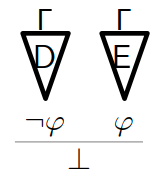
\includegraphics[width=.5\linewidth]{Assets/Logik-Negationselimination.png}
\end{flashcard}

\begin{flashcard}[ Natürliches Schließen ]{ Falsum }
    ex falso sequitur quodlibet\newline
    ausführlich: Ist D eine Deduktion von $\bot$ mit Hypothesen aus $\Gamma$, so ergibt sich die folgende Deduktion von $\varphi$ mit Hypothesen aus $\Gamma$:
    \begin{prooftree}
        \AxiomC{$\bot$}
        \RightLabel{\scriptsize ($\bot$)}
        \UnaryInfC{$\varphi$}
    \end{prooftree}
    %\includegraphics[width=.5\linewidth]{Assets/Logik-Falsumeinführung.png}
\end{flashcard}

\begin{flashcard}[ Natürliches Schließen ]{ reductio ad absurdum }
    Ist D eine Deduktion von $\bot$ mit Hypothesen aus $\Gamma\cup\{\lnot\varphi\}$, so ergibt sich die folgende Deduktion von $\varphi$ mit Hypothesen aus $\Gamma$:
    \begin{prooftree}
        \AxiomC{[$\lnot\varphi$]}\noLine
        \UnaryInfC{$\bot$}
        \RightLabel{\scriptsize ($\bot$)}
        \UnaryInfC{$\varphi$}
    \end{prooftree}
    %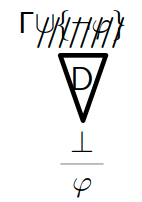
\includegraphics[width=.5\linewidth]{Assets/Logik-reductio-ad-absurdum.png}
\end{flashcard}

\begin{flashcard}[ Natürliches Schließen ]{ $\Gamma\Vdash\varphi$ }
    Für eine Formelmenge $\Gamma$ und eine Formel $\varphi$ schreiben wir $\Gamma\Vdash\varphi$ wenn es eine Deduktion gibt mit Hypothesen aus $\Gamma$ und Konklusion $\varphi$. Wir sagen "$\varphi$ ist eine syntaktische Folgerung von $\Gamma$".

    Eine Formel $\varphi$ ist ein Theorem, wenn $\varnothing\Vdash\varphi$ gilt.

    $\Gamma\Vdash\varphi$ sagt (zunächst) nichts über den Inhalt der Formeln in $\Gamma\cup\{\varphi\}$ aus, sondern nur über die Tatsache, dass $\varphi$ mithilfe des natürlichen Schließens aus den Formeln aus $\Gamma$ hergeleitet werden kann.

    Ebenso sagt "$\varphi$ ist Theorem" nur, dass $\varphi$ abgeleitet werden kann, über "Wahrheit" sagt dieser Begriff (zunächst) nichts aus.
\end{flashcard}

\begin{flashcard}[ Natürliches Schließen ]{ $\lnot(\varphi\vee\psi)$ }
    Für alle Formeln $\varphi$ und $\psi$ gilt $\{\lnot(\varphi\vee\psi)\}\Vdash\lnot\varphi\wedge\lnot\psi$.
\end{flashcard}

\begin{flashcard}[ Natürliches Schließen ]{ $\lnot\lnot\varphi$ }
    Für jede Formel $\varphi$ ist $\lnot\lnot\varphi\rightarrow\varphi$ ein Theorem.
\end{flashcard}

\begin{flashcard}[ Natürliches Schließen ]{ Für jede Formel $\varphi$ ist $\varphi\vee\lnot\varphi$... }
    Für jede Formel $\varphi$ ist $\varphi\vee\lnot\varphi$ ein Theorem.

    Beweis: Wir geben eine Deduktion mit Konklusion $\varphi\vee\lnot\varphi$ ohne Hypothesen an...
\end{flashcard}

\begin{flashcard}[ Natürliches Schließen ]{ $\{\lnot(\varphi\wedge\psi)\}\Vdash ...$ }
    $\{\lnot(\varphi\wedge\psi)\}\Vdash\lnot\varphi\vee\lnot\psi$
\end{flashcard}

\begin{flashcard}[ Semantik ]{ Idee der Semantik }
    wenn man jeder atomaren Formel $p_i$ einen Wahrheitswertzuordnet, so kann man den Wahrheitswert jeder Formel berechnen.
\end{flashcard}

\begin{flashcard}[ Semantik ]{ zweiwertige Logik }
    Boolesche Logik $B=\{0,1\}$

    Wahrheitswerte ,,wahr''=1 und ,,falsch''= 0
\end{flashcard}

\begin{flashcard}[ Semantik ]{ dreiwertige Logik }
    Kleene-Logik $K_3=\{0,\frac{1}{2},1\}$:

    zusätzlicher Wahrheitswert ,,unbekannt'' $=\frac{1}{2}$
\end{flashcard}

\begin{flashcard}[ Semantik ]{ Fuzzy-Logik }
    $F=[0,1]$: Wahrheitswerte sind ,,Grad der Überzeugtheit''
\end{flashcard}

\begin{flashcard}[ Semantik ]{ unendliche Boolesche Algebra }
    $B_R$= Menge der Teilmengen von $\mathbb{R}$;

    $A\subseteq\mathbb{R}$ ist ,,Menge der Menschen, die Aussage für wahr halten''
\end{flashcard}

\begin{flashcard}[ Semantik ]{ Heyting-Algebra }
    $H_R$= Menge der offenen Teilmengen von $\mathbb{R}$

    Erinnerung: $A\subseteq\mathbb{R}$ offen, wenn $\forall a\in A\exists\epsilon >0:(a-\epsilon,a+\epsilon)\subseteq A$, d.h. wenn $A$ abzählbare Vereinigung von offenen Intervallen $(x,y)$ ist.
\end{flashcard}

\begin{flashcard}[ Semantik ]{ offen vs. nicht offene Teilmengen }
    offen: $(0,1), \mathbb{R}_{>0}, \mathbb{R}\backslash\{0\}, \mathbb{R}\backslash\mathbb{N}$

    nicht offen: $[1,2), \mathbb{R}_{\geq 0}, \mathbb{Q}, \mathbb{N}, \{\frac{1}{n} | n\in\mathbb{N}\}, \mathbb{R}\backslash\mathbb{Q}$
\end{flashcard}

\begin{flashcard}[ Semantik ]{ W-Belegung }
    Sei W eine Menge von Wahrheitswerten.

    Eine W-Belegung ist eine Abbildung $B:V\rightarrow W$, wobei $V\subseteq\{p_0 ,p_1 ,...\}$ eine Menge atomarer Formeln ist.

    Die W-Belegung $B:V\rightarrow W$ paßt zur Formel $\phi$, falls alle atomaren Formeln aus $\phi$ zu V gehören.
\end{flashcard}

\begin{flashcard}[ Wahrheitswertebereiche ]{ Definition: Sei W eine Menge und $R\subseteq W\times W$ eine binäre Relation. }
    Sei W eine Menge und $R\subseteq W\times W$ binäre Relation.
    \begin{itemize*}
        \item R ist reflexiv
        \item R ist antisymmetrisch
        \item R ist transitive
        \item R ist eine Ordnungsrelation
    \end{itemize*}
\end{flashcard}

\begin{flashcard}[ Wahrheitswertebereiche ]{ reflexive Relation }
    R ist reflexiv, wenn $(a,a)\in R$ für alle $a\in W$ gilt.
\end{flashcard}

\begin{flashcard}[ Wahrheitswertebereiche ]{ antisymmetrische Relation }
    R ist antisymmetrisch, wenn $(a,b),(b,a)\in R$ impliziert, dass $a=b$ gilt (für alle $a,b\in W$).
\end{flashcard}

\begin{flashcard}[ Wahrheitswertebereiche ]{ transitive Relation }
    R ist transitive, wenn $(a,b),(b,c)\in R$ impliziert, dass $(a,c)\in R$ gilt (für alle $a,b,c\in W$).
\end{flashcard}

\begin{flashcard}[ Wahrheitswertebereiche ]{ Ordnungsrelation }
    R ist eine Ordnungsrelation, wenn R reflexiv, antisymmetrisch und transitiv ist. In diesem Fall heißt das Paar $(W,R)$ eine partiell geordnete Menge.
\end{flashcard}

\begin{flashcard}[ Wahrheitswertebereiche ]{ Schranken }
    $(W,\leq)$ partiell geordnete Menge, $M\subseteq W$ und $a\in W$
    \begin{itemize*}
        \item a ist obere Schranke von $M$, wenn $m\leq a$...
        \item a ist kleinste obere Schranke oder Supremum...
        \item a ist untere Schranke von $M$, wenn $a\leq m$...
        \item a ist größte untere Schranke oder Infimum...
    \end{itemize*}
\end{flashcard}

\begin{flashcard}[ Wahrheitswertebereiche ]{ obere Schranke }
    $(W,\leq)$ partiell geordnete Menge, $M\subseteq W$ und $a\in W$

    a ist obere Schranke von $M$, wenn $m\leq a$ für alle $m\in M$ gilt
\end{flashcard}

\begin{flashcard}[ Wahrheitswertebereiche ]{ kleinste obere Schranke  }
    $(W,\leq)$ partiell geordnete Menge, $M\subseteq W$ und $a\in W$

    a ist kleinste obere Schranke/Supremum von $M$, wenn $a$ obere Schranke von $M$ ist und wenn $a\leq b$ für alle oberen Schranken $b$ von $M$ gilt. Wir schreiben in diesem Fall $a=sup\ M$.

    z.B. $(W,\leq)$ mit $W=R$ und $\leq$ übliche Ordnung auf R
    \begin{itemize*}
        \item dann gelten sup[0, 1] = sup(0, 1) = 1.
        \item $sup\ W$ existiert nicht (W keine obere Schranke)
    \end{itemize*}
\end{flashcard}

\begin{flashcard}[ Wahrheitswertebereiche ]{ untere Schranke }
    Sei $(W,\leq)$ partiell geordnete Menge, $M\subseteq W$ und $a\in W$.

    a ist untere Schranke von $M$, wenn $a\leq m$ für alle $m\in M$ gilt.
\end{flashcard}

\begin{flashcard}[ Wahrheitswertebereiche ]{ größte untere Schranke }
    Sei $(W,\leq)$ partiell geordnete Menge, $M\subseteq W$ und $a\in W$.

    a ist größte untere Schranke oder Infimum von $M$, wenn a untere Schranke von $M$ ist und wenn $b\leq a$ für alle unteren Schranken $b$ von $M$ gilt. Wir schreiben in diesem Fall $a=inf\ M$.
\end{flashcard}

\begin{flashcard}[ Wahrheitswertebereiche ]{ (vollständiger) Verband }
    Ein (vollständiger) Verband ist eine partiell geordnete Menge $(W,\leq)$, in der jede Menge $M\subseteq W$ ein Supremum $sup\ M$ und ein Infimum $inf\ M$ hat. In einem Verband $(W,\leq)$ definieren wir:
    \begin{itemize*}
        \item $0_W = inf\ W$ und $1_W= sup\ W$
        \item $a\wedge_W b= inf\{a,b\}$ und $a\vee_W b= sup\{a,b\}$ für $a,b\in W$
    \end{itemize*}
    In jedem Verband $(W,\leq)$ gelten $0_W= sup\ \varnothing$ und $1_W= inf\ \varnothing$ (denn jedes Element von $W$ ist obere und untere Schranke von $\varnothing$).
\end{flashcard}

\begin{flashcard}[ Wahrheitswertebereiche ]{ Wahrheitswertebereich (Tupel?) }
    Ein Wahrheitswertebereich ist ein Tupel $(W,\leq,\rightarrow W,\lnot W)$, wobei $(W,\leq)$ ein Verband und $\rightarrow W:W^2 \rightarrow W$ und $\lnot W:W\rightarrow W$  Funktionen sind.
\end{flashcard}

\begin{flashcard}[ Wahrheitswertebereiche ]{ Boolesche Wahrheitswertebereich $B$ }
    Der Boolesche Wahrheitswertebereich B ist definiert durch die Grundmenge $B=\{0,1\}$, die natürliche Ordnung $\leq$ und die Funktionen $\lnot_B (a) = 1-a$, $\rightarrow_B(a,b) = max(b, 1 -a)$. Hier gelten:
    \begin{itemize*}
        \item $0_B=0$, $1_B= 1$,
        \item $a\wedge_B b= min(a,b)$, $a\vee_B b= max(a,b)$
    \end{itemize*}
\end{flashcard}

\begin{flashcard}[ Wahrheitswertebereiche ]{ Kleenesche Wahrheitswertebereich }
    Der Kleenesche Wahrheitswertebereich $K_3$ ist definiert durch die Grundmenge $K_3=\{0,\frac{1}{2},1\}$ mit der natürlichen Ordnung $\leq$ und durch die Funktionen $\lnot_{K_3} (a) = 1 -a $, $\rightarrow_{K_3} (a,b) = max(b, 1-a)$. Hier gelten:
    \begin{itemize*}
        \item $\lnot_{K_3} = 0$, $1_{K_3} = 1$
        \item $a\wedge_{K_3} b= min(a,b)$, $a\vee_{K_3} b= max(a,b)$
    \end{itemize*}
\end{flashcard}

\begin{flashcard}[ Wahrheitswertebereiche ]{ Wahrheitswertebereiche Fuzzy-Logik }
    Der Wahrheitswertebereich F der Fuzzy-Logik ist definiert durch die Grundmenge $F=[0,1]\subseteq\mathbb{R}$ mit der natürlichen Ordnung $\leq$ und durch die Funktionen $\lnot_F (a) = 1-a$, $\rightarrow_F (a,b) = max(b, 1-a)$. Hier gelten:
    \begin{itemize*}
        \item $0_F= 0$, $1_F= 1$
        \item $a\wedge_F b= min(a,b)$, $a\vee_F b= max(a,b)$
    \end{itemize*}
\end{flashcard}

\begin{flashcard}[ Wahrheitswertebereiche ]{ Boolesche Wahrheitswertebereich $B_R$ }
    Der Boolesche Wahrheitswertebereich $B_R$ ist definiert durch die Grundmenge $B_R=\{A|A\subseteq \mathbb{R}\}$ mit der Ordnung $\subseteq$ und durch die Funktionen $\lnot_{B_R} (A) =\mathbb{R}\backslash A$, $\rightarrow_{B_R} (A,B) = B\cup\mathbb{R}\backslash A$. Hier gelten:
    \begin{itemize*}
        \item $0_{B_R}=\varnothing$, $1_{B_R}=\mathbb{R}$
        \item $A\wedge_{B_R} B=A\cap B$, $A\vee_{B_R} B=A\cup B$
    \end{itemize*}
\end{flashcard}

\begin{flashcard}[ Wahrheitswertebereiche ]{ Heytingsche Wahrheitswertebereich $H_R$ }
    Der Heytingsche Wahrheitswertebereich $H_R$ ist definiert durch die Grundmenge $H_{\mathbb{R}} =\{A\subseteq\mathbb{R} | \text{A ist offen}\}$, die Ordnung $\subseteq$ und durch die Funktionen $\lnot_{H_R} (A) = Inneres(\mathbb{R}\backslash A)$, $\rightarrow_{H_R} (A,B) =Inneres(B\cup \mathbb{R}\backslash A)$. Hier gelten:
    \begin{itemize*}
        \item $0_{H_R}=\varnothing$, $1_{H_R}=\mathbb{R}$
        \item $A\wedge_{H_R} B= A\cap B$, $A\vee_{H_R} B=A\cup B$
        \item $Inneres(A) =\{a\in A|\exists \epsilon >0 : (a-\epsilon,a+\epsilon)\subseteq A\}$
    \end{itemize*}
\end{flashcard}

\begin{flashcard}[ Wahrheitswertebereiche ]{ $\hat{B}(\phi)\in W$ jeder zu $B$ passenden Formel $\phi$}
    W Wahrheitswertebereich und B W-Belegung. Über Formelaufbau definieren wir Wahrheitswert $\hat{B}(\phi)\in W$ jeder zu $B$ passenden Formel $\phi$:
    \begin{itemize*}
        \item $\hat{B}(\bot) = 0_W$
        \item $\hat{B}(p) = B(p)$ falls $p$ eine atomare Formel ist
        \item $\hat{B}((\phi\wedge \psi )) = \hat{B}(\phi)\wedge_W \hat{B}(\psi )$
        \item $\hat{B}((\phi\vee \psi )) = \hat{B}(\phi)\vee_W \hat{B}(\psi )$
        \item $\hat{B}((\phi\rightarrow \psi )) = \rightarrow W(\hat{B}(\phi),\hat{B}(\psi ))$
        \item $\hat{B}(\lnot\phi) = \lnot W(\hat{B}(\phi))$
    \end{itemize*}
\end{flashcard}

\begin{flashcard}[ Wahrheitswertebereiche ]{ W-Folgerung }
    Sei W ein Wahrheitswertebereich.
    Eine Formel $\phi$ heißt eine W-Folgerung der Formelmenge $\Gamma$, falls für jede W-Belegung B, die zu allen Formeln aus $\Gamma \cup\{\phi\}$ paßt, gilt:
    $inf\{B(\gamma )|\gamma \in \Gamma \}\leq B(\phi)$

    Wir schreiben $\Gamma \Vdash W\phi$, falls $\phi$ eine W-Folgerung von $\Gamma$ ist.

    Bemerkung: Im Gegensatz zur Beziehung $\Gamma \vdash \phi$, d.h. zur syntaktischen Folgerung, ist $\Gamma \Vdash W \phi$ eine semantische Beziehung.
\end{flashcard}

\begin{flashcard}[ Wahrheitswertebereiche ]{ W-Tautologie }
    Eine W-Tautologie ist eine Formel $\phi$ mit $\varnothing \Vdash W\phi$, d.h. $B(\phi) = 1_W$ für alle passenden W-Belegungen B (denn $inf\{\hat{B}(\gamma )|\gamma \in \varnothing \}= inf \varnothing = 1_W)$.
\end{flashcard}

\begin{flashcard}[ Wahrheitswertebereiche ]{ $\varnothing\Vdash_W\lnot\lnot\phi\rightarrow\phi$ gilt für Wahrheitsbereiche... }
    $B, B_{\mathbb{R}}$
\end{flashcard}

\begin{flashcard}[ Wahrheitswertebereiche ]{ $\varnothing\Vdash_W\phi\vee\lnot\phi$  }
    $B, B_{\mathbb{R}}$
\end{flashcard}

\begin{flashcard}[ Wahrheitswertebereiche ]{ $\{\lnot\phi\rightarrow\bot\}\Vdash_W\phi$ gilt für Wahrheitsbereiche...  }
    $B, B_{\mathbb{R}}, K_3, F$
\end{flashcard}

\begin{flashcard}[ Wahrheitswertebereiche ]{ $\{\phi\}\Vdash_W\lnot\phi\rightarrow\bot$ gilt für Wahrheitsbereiche...  }
    $B, B_{\mathbb{R}}, K_3, F, H_{\mathbb{R}}$
\end{flashcard}

\begin{flashcard}[ Wahrheitswertebereiche ]{ syntaktische Folgerung }
    $\Gamma\vdash\phi$ syntaktische Folgerung
\end{flashcard}

\begin{flashcard}[ Wahrheitswertebereiche ]{ Theorem }
    Theorem = ,,hypothesenlos ableitbar''
\end{flashcard}

\begin{flashcard}[ Wahrheitswertebereiche ]{ W-Tautologie }
    W-Tautologie = ,,wird immer zu $1_W$ ausgewertet''
\end{flashcard}

\begin{flashcard}[ Wahrheitswertebereiche ]{ (semantische) W-Folgerung }
    $\Gamma\Vdash_W \phi$ (semantische) W-Folgerung
\end{flashcard}

\begin{flashcard}[ Korrekheit ]{ Frage der Korrektheit }
    Können wir durch mathematische Beweise zu falschen Aussagenkommen?
    Können wir durch das natürliche Schließen zu falschen Aussagen kommen?

    Existiert eine Menge $\Gamma$ von Formeln und eine Formel $\varphi$ mit $\Gamma\vdash\varphi$ und $\Gamma\not\Vdash_W \varphi$? Für welche Wahrheitswertebereiche W?

    Für welche Wahrheitswertebereiche W gilt $$\Gamma\vdash\varphi\Rightarrow\Gamma\vdash_W \varphi$$ bzw. $\varphi$ ist Theorem $\Rightarrow\varphi$ ist W-Tautologie?
\end{flashcard}

\begin{flashcard}[ Korrekheit ]{ Korrektheitslemma für nat. Schließen \& Wahrheitswertebereich B }
    Sei $D$ eine Deduktion mit Hypothesen in der Menge $\Gamma$ und Konklusion $\varphi$. Dann gilt $\Gamma\vdash_B \varphi$, d.h. $inf\{B(\gamma)|\gamma\in\Gamma\}\leq B(\varphi)$ für alle passenden B-Belegungen $B$.
\end{flashcard}

\begin{flashcard}[ Korrekheit ]{ Korrektheitssatz für natürliches Schließen \& Wahrheitswertebereich $B$ }
    Für jede Menge von Formeln $\Gamma$ und jede Formel $\varphi$ gilt $\Gamma\vdash\varphi\Rightarrow\Gamma\vdash_B\varphi$.

    Beweis: Wegen $\Gamma\vdash\varphi$ existiert eine Deduktion $D$ mit Hypothesen in $\Gamma$ und Konklusion $\varphi$. Nach dem Korrektheitslemma folgt $\Gamma\vdash_B \varphi$.
\end{flashcard}

\begin{flashcard}[ Korrekheit ]{ Jedes Theorem ist eine B-Tautologie? }
    wahr
\end{flashcard}

\begin{flashcard}[ Korrekheit ]{ Korrektheitssatz für natürliches Schließen \& Wahrheitswertebereich $B_\mathbb{R}$}
    Für jede Menge von Formeln $\Gamma$ und jede Formel $\varphi$ gilt  $\Gamma\vdash\varphi\Rightarrow\Gamma\vdash_{B_\mathbb{R}}\varphi$.
    Definition
\end{flashcard}

\begin{flashcard}[ Korrekheit ]{ Jedes Theorem ist eine $B_\mathbb{R}$-Tautologie? }
    wahr
\end{flashcard}

\begin{flashcard}[ Korrekheit ]{ Korrektheitslemma für nat. Schließen \& Wahrheitswertebereich  $H_{\mathbb{R}}$ }
    Sei $D$ eine Deduktion mit Hypothesen in der Menge $\Gamma$ und Konklusion $\varphi$, die die Regel $(raa)$ nicht verwendet. Dann gilt $\Gamma\vdash_{H_\mathbb{R}}\varphi$.

\end{flashcard}

\begin{flashcard}[ Korrekheit ]{ Korrektheitssatz für nat. Schließen \& Wahrheitswertebereich  $H_{\mathbb{R}}$ }
    Für jede Menge von Formeln $\Gamma$ und jede Formel $\varphi$ gilt $\Gamma\vdash\varphi$ ohne $(raa)$ $\Rightarrow\Gamma\vdash_{H_{\mathbb{R}}}\varphi$
\end{flashcard}

\begin{flashcard}[ Korrekheit ]{ Jedes $(raa)$-frei herleitbare Theorem ist eine $H_{\mathbb{R}}$-Tautologie? }
    wahr
\end{flashcard}

\begin{flashcard}[ Korrekheit ]{ Deduktion von Thermen ohne Hypothesen mit (raa) }
    Jede Deduktion der Theoreme $\lnot\lnot\varphi\rightarrow\varphi$ und $\varphi\vee\lnot\varphi$ ohne Hypothesen verwendet $(raa)$.
\end{flashcard}

\begin{flashcard}[ Vollständigkeit ]{ Frage der Vollständigkeit }
    Können wir durch mathematische Beweise zu allen korrekten Aussagen kommen?
    Können wir durch das natürliche Schließen zu allen korrekten Aussagen kommen?

    Existiert eine Menge $\Gamma$ von Formeln und eine Formel $\varphi$ mit $\Gamma\vdash_W\varphi$ und $\Gamma\not\vdash\varphi$? Für welche Wahrheitswertebereiche $W$?
    Für welche Wahrheitswertebereiche $W$ gilt $\Gamma\vdash_W \varphi\Rightarrow\Gamma\vdash\varphi$ bzw. $\varphi$ ist $W$-Tautologie $\Rightarrow\varphi$ ist Theorem?

\end{flashcard}

\begin{flashcard}[ Vollständigkeit ]{ Konsistente Mengen }
    Sei $\Gamma$ eine Menge von Formeln. $\Gamma$ heißt inkonsistent, wenn $\Gamma\vdash\bot$ gilt. Sonst heißt $\Gamma$ konsistent.
\end{flashcard}

\begin{flashcard}[ Vollständigkeit ]{ Lemma konsistente Menge }
    Sei $\Gamma$ eine Menge von Formeln und $\varphi$ eine Formel. Dann gilt $\Gamma\not\vdash\varphi \Leftrightarrow \Gamma\cup\{\lnot\varphi\}$ konsistent.
\end{flashcard}

\begin{flashcard}[ Vollständigkeit ]{ Maximal konsistente Mengen }
    Eine Formelmenge $\Delta$ ist maximal konsistent, wenn sie konsistent ist und wenn gilt ,,$\sum\supseteq\Delta$ konsistent $\Rightarrow\sum = \Delta$''.
\end{flashcard}

\begin{flashcard}[ Vollständigkeit ]{ Satz maximal konsistene Menge }
    Jede konsistente Formelmenge $\Gamma$ ist in einer maximal konsistenten Formelmenge $\Delta$ enthalten.
\end{flashcard}

\begin{flashcard}[ Vollständigkeit ]{ Sei $\Delta$ maximal konsistent und gelte $\Delta\vdash\varphi$ }
    Sei $\Delta$ maximal konsistent und gelte $\Delta\vdash\varphi$. Dann gilt $\varphi\in\Delta$.
\end{flashcard}

\begin{flashcard}[ Vollständigkeit ]{ Sei $\Delta$ maximal konsistent und $\varphi$ Formel }
    Sei $\Delta$ maximal konsistent und $\varphi$ Formel. Dann gilt $\varphi\not\in\Delta\Leftrightarrow\lnot\varphi\in\Delta$.
\end{flashcard}

\begin{flashcard}[ Erfüllbare Mengen ]{ $\Gamma$ heißt erfüllbar, wenn }
    Sei $\Gamma$ eine Menge von Formeln. $\Gamma$ heißt erfüllbar, wenn es eine passende B-Belegung $B$ gibt mit $B(\gamma) = 1_B$ für alle $\gamma\in\Gamma$.

    Die Erfüllbarkeit einer endlichen Menge $\Gamma$ ist entscheidbar (NP-vollständig)
\end{flashcard}

\begin{flashcard}[ Erfüllbare Mengen ]{ $Delta$ maximal konsistente Menge }
    Sei $\Delta$ eine maximal konsistente Menge von Formeln. Dann ist $\Delta$ erfüllbar.
\end{flashcard}

\begin{flashcard}[ Erfüllbare Mengen ]{ $\Gamma\not\Vdash_B\varphi\Leftrightarrow...$ }
    Sei $\Gamma$ eine Menge von Formeln und $\varphi$ eine Formel. Dann gilt $\Gamma\not\Vdash_B\varphi\Leftrightarrow\Gamma\cup\{\lnot \varphi\}$ erfüllbar.
\end{flashcard}

\begin{flashcard}[ Erfüllbare Mengen ]{ $\Gamma\Vdash W\varphi\Rightarrow...$ }
    Sei $W$ einer der Wahrheitswertebereiche $B, K_3, F, H_R$ und $B_R,\Gamma$ eine Menge von Formeln und $\varphi$ eine Formel. Dann gilt $\Gamma\Vdash W\varphi\Rightarrow\Gamma\Vdash B\varphi$.
\end{flashcard}

\begin{flashcard}[ Erfüllbare Mengen ]{ Vollständigkeitssatz }
    Sei $\Gamma$ eine Menge von Formeln, $\varphi$ eine Formel und $W$ einer der Wahrheitswertebereiche $B,K_3 , F, B_R$ und $H_R$. Dann gilt $\Gamma\Vdash_W\varphi \Rightarrow \Gamma\vdash\varphi$.

    Insbesondere ist jede W-Tautologie ein Theorem.
\end{flashcard}

\begin{flashcard}[ Vollständigkeit und Korrektheit ]{ Satz $\Gamma\vdash\varphi\Leftrightarrow\Gamma\Vdash_B \varphi$}
    Seien $\Gamma$ eine Menge von Formeln und $\varphi$ eine Formel. Dann gilt $$\Gamma\vdash\varphi\Leftrightarrow\Gamma\Vdash_B \varphi$$
    Insbesondere ist eine Formel genau dann eine B-Tautologie, wenn sie ein Theorem ist.
    \begin{itemize*}
        \item gilt für jede ,,Boolesche Algebra'', z.B. $B_R$
        \item $\Gamma\vdash\varphi$ ohne ($raa$) $\Leftrightarrow\Gamma\Vdash_{H_R} \varphi$ (Tarksi 1938)
    \end{itemize*}
\end{flashcard}

\begin{flashcard}[ Entscheidbarkeit ]{ Satz Menge der Theoreme }
    Satz: die Menge der Theoreme ist entscheidbar.
\end{flashcard}

\begin{flashcard}[ Vollständigkeit und Korrektheit ]{ Äquivalenzen und Theoreme }
    Zwei Formeln $\alpha$ und $\beta$ heißen äquivalent $(\alpha\equiv\beta)$, wenn für alle passenden B-Belegungen $B$ gilt: $B(\alpha) =B(\beta)$.
\end{flashcard}

\begin{flashcard}[ Vollständigkeit und Korrektheit ]{ Liste der Äquivalenzen 1/2 }
    Es gelten die folgenden Äquivalenzen:
    \begin{enumerate*}
        \item $p_1 \vee p_2 \equiv p_2 \vee p_1$
        \item $(p_1 \vee p_2 )\vee p_3 \equiv p_1 \vee (p_2 \vee p_3 )$
        \item $p_1 \vee (p_2 \wedge p_3 )\equiv (p_1 \vee p_2 )\wedge (p_1 \vee p_3 )$
        \item $\lnot(p_1 \vee p_2 )\equiv\lnot p_1 \wedge\lnot p_2$
        \item $p_1 \vee p_1 \equiv p_1$
    \end{enumerate*}
    Bemerkung: Mit den üblichen Rechenregeln für Gleichungen können aus dieser Liste alle gültigen Äquivalenzen hergeleitet werden.
\end{flashcard}

\begin{flashcard}[ Vollständigkeit und Korrektheit ]{ Liste der Äquivalenzen 2/2 }
    Es gelten die folgenden Äquivalenzen:
    \begin{enumerate*}
        \item  $(p_1 \wedge \lnot p_1 )\vee p_2 \equiv p_2$
        \item  $\lnot\lnot p_1\equiv p_1$
        \item  $p_1 \wedge\lnot p_1 \equiv\bot$
        \item  $p_1 \vee\lnot p_1 \equiv\lnot\bot$
        \item  $p_1 \rightarrow p_2 \equiv \lnot p_1 \vee p_2$
    \end{enumerate*}
    Bemerkung: Mit den üblichen Rechenregeln für Gleichungen können aus dieser Liste alle gültigen Äquivalenzen hergeleitet werden.
\end{flashcard}

\begin{flashcard}[ Vollständigkeit und Korrektheit ]{ Zusammenhang zw. Theoremen und Äquivalenzen }
    Seien $\alpha$ und $\beta$ zwei Formeln. Dann gilt $\alpha\equiv\beta\Leftrightarrow(\alpha\leftrightarrow\beta)$ ist Theorem.
\end{flashcard}

\begin{flashcard}[ Vollständigkeit und Korrektheit ]{ $\alpha$ ist Theorem $\Leftrightarrow\alpha\equiv\lnot\bot$ }
    Sei $\alpha$ eine Formel. Dann gilt $\alpha$ ist Theorem $\Leftrightarrow\alpha\equiv\lnot\bot$.
\end{flashcard}

\begin{flashcard}[ Kompaktheitsatzes ]{ Kompaktheit }
    Sei $\Gamma$ eine u.U. unendliche Menge von Formeln und $\varphi$ eine Formel mit $\Gamma\Vdash_B\varphi$. Dann existiert $\Gamma'\subseteq\Gamma$ endlich mit $\Gamma'\Vdash_B \varphi$.
\end{flashcard}

\begin{flashcard}[ Kompaktheitsatzes ]{ Kompaktheits- oder Endlichkeitssatz }
    Sei $\Gamma$ eine u.U. unendliche Menge von Formeln. Dann gilt $\Gamma$ unerfüllbar $\Leftrightarrow\exists\Gamma'\subseteq\Gamma$ endlich: $\Gamma'$ unerfüllbar
\end{flashcard}

\begin{flashcard}[ Kompaktheitsatzes ]{ Färbbarkeit }
    Ein Graph ist ein Paar $G=(V,E)$ mit einer Menge $V$
    und $E\subseteq\binom{V}{2} =\{X\subseteq V:|V\Vdash 2 \}$.
    Für $W\subseteq V$ sei $G\upharpoonright_W= (W,E\cap\binom{W}{2})$ der von $W$ induzierte Teilgraph.
    Der Graph G ist 3-färbbar, wenn es eine Abbildung $f:V\rightarrow\{1,2,3\}$ mit $f(v)\not=f(w)$ für alle $\{v,w\}\in E$.

    Bemerkung: Die 3-Färbbarkeit eines endlichen Graphen ist NP-vollständig
\end{flashcard}

\begin{flashcard}[ Kompaktheitsatzes ]{ Sei $G= (N,E)$ ein Graph }
    Sei $G= (N,E)$ ein Graph. Dann sind äquivalent
    \begin{enumerate*}
        \item $G$ ist 3-färbbar.
        \item Für jede endliche Menge $W\subseteq N$ ist $G\upharpoonright_W$ 3-färbbar.
    \end{enumerate*}
\end{flashcard}

\begin{flashcard}[ Kompaktheitsatzes ]{ Parkettierungen Idee }
    Gegeben ist eine Menge von quadratischen Kacheln mit gefärbten Kanten. Ist es möglich, mit diesen Kacheln die gesamte Ebene zu füllen, so dass aneinanderstoßende Kanten gleichfarbig sind?
\end{flashcard}

\begin{flashcard}[ Kompaktheitsatzes ]{ Kachelsystem Definition }
    Ein Kachelsystem besteht aus einer endlichen Menge C von ,,Farben'' und einer Menge K von Abbildungen $\{N,O,S,W\}\rightarrow C$ von ,,Kacheln''.

    Eine Kachelung von $G\subseteq Z\times Z$ ist eine Abbildung $f:G\rightarrow K$ mit
    \begin{itemize*}
        \item $f(i,j)(N) =f(i,j+ 1 )(S)$ für alle $(i,j),(i,j+ 1 )\in G$
        \item $f(i,j)(O) =f(i+ 1 ,j)(W)$ für alle $(i,j),(i+ 1 ,j)\in G$
    \end{itemize*}
\end{flashcard}

\begin{flashcard}[ Kompaktheitsatzes ]{ Kachelsystem Satz }
    Sei $K$ ein Kachelsystem. Es existiert genau dann eine Kachelung von $Z\times Z$, wenn für jedes $n\in N$ eine Kachelung von $\{(i,j) :|i|,|j| \leq n\}$ existiert.
\end{flashcard}

\begin{flashcard}[ Erfüllbarkeit ]{ Erfüllbarkeitsproblem }
    Eingabe: Formel $\Gamma$

    Frage: existiert eine B-Belegung $B$ mit $B(\Gamma) = 1_B$.
\end{flashcard}

\begin{flashcard}[ Erfüllbarkeit ]{ Hornklausel }
    Eine Hornklausel hat die Form $(\lnot\bot\wedge p_1\wedge p_2\wedge ... \wedge p_n)\rightarrow q$ für $n\geq 0$, atomare Formeln $p_1 ,p_2 ,... ,p_n$ und $q$ atomare Formel oder $q=\bot$. In der Literatur auch:
    \begin{itemize*}
        \item $\{\lnot p_1,\lnot p_2 ,... ,\lnot p_n,q\}$ für $\{p_1 ,... ,p_n\}\rightarrow q$ mit $q$ atomare Formel
        \item $\{\lnot p_1,\lnot p_2 ,... ,\lnot p_n\}$ für $\{p_1 ,... ,p_n\}\rightarrow\bot$
        \item $\Box$ für $\varnothing\rightarrow\bot$, die ,,leere Hornklausel''
    \end{itemize*}
\end{flashcard}

\begin{flashcard}[ Erfüllbarkeit ]{ Hornformel }
    Eine Hornformel ist eine Konjunktion von Hornklauseln.
\end{flashcard}

\begin{flashcard}[ Erfüllbarkeit ]{ Markierungsalgorithmus }
    Eingabe: eine endliche Menge $\Gamma$ von Hornklauseln.
    \begin{enumerate*}
        \item \textbf{while} es gibt in $\Gamma$ eine Hornklausel $M\rightarrow q$, so daß alle $p\in M$ markiert sind und $q$ unmarkierte atomare Formel ist $\Rightarrow$ \textbf{do} markiere $q$ (in allen Hornklauseln in $\Gamma$)
        \item \textbf{if} $\Gamma$ enthält eine Hornklausel der Form $M\rightarrow\bot$, in der alle $p\in M$ markiert sind
        \textbf{then} return ,,unerfüllbar''
        \textbf{else} return ,,erfüllbar''
    \end{enumerate*}
\end{flashcard}

\begin{flashcard}[ Erfüllbarkeit ]{ Terminierung endlicher Menge von Hornklauseln }
    Sei $\Gamma$ endliche Menge von Hornklauseln. Dann terminiert der Markierungsalgorithmus mit dem korrekten Ergebnis.
\end{flashcard}

\begin{flashcard}[ Erfüllbarkeit ]{ SLD-Resolution Definition }
    Sei $\Gamma$ eine Menge von Hornklauseln. Eine SLD-Resolution aus $\Gamma$ ist eine Folge $(M_0\rightarrow\bot,M_1\rightarrow\bot,... ,M_m\rightarrow\bot)$ von Hornklauseln mit
    \begin{itemize*}
        \item $(M_0\rightarrow\bot)\in\Gamma$
        \item für alle $0\leq n<m$ existiert $(N\rightarrow q)\in\Gamma$ mit $q\in M_n$ und $M_{n+1} = M_n\backslash\{q\}\cup N$
    \end{itemize*}
\end{flashcard}

\begin{flashcard}[ Erfüllbarkeit ]{ SLD-Resolution Beispiel \newline $\Gamma =\{\{BH\}\rightarrow AK,\{AK,BH\}\rightarrow\bot,\{RL,AK\}\rightarrow BH,\varnothing\rightarrow RL,\varnothing\rightarrow AK\}$}
    \begin{itemize*}
        \item $M_0 =\{AK,BH\}$
        \item $M_1 =M_0 \backslash\{BH\}\cup\{RL,AK\}=\{RL,AK\}$
        \item $M_2 =M_1 \backslash\{RL\}\cup\varnothing =\{AK\}$
        \item $M_3 =M_2 \backslash\{AK\}\cup\varnothing =\varnothing$
    \end{itemize*}
\end{flashcard}

\begin{flashcard}[ Erfüllbarkeit ]{ Lemma A: $\Gamma$ nicht erfüllbar }
    Sei $\Gamma$ eine (u.U. unendliche) Menge von Hornklauseln und $(M_0\rightarrow\bot, M_1\rightarrow\bot,... , M_m\rightarrow\bot)$ eine SLD-Resolution aus $\Gamma$ mit $M_m=\varnothing$. Dann ist $\Gamma$ nicht erfüllbar.
\end{flashcard}

\begin{flashcard}[ Erfüllbarkeit ]{ Lemma B: SLD Resolution existiert }
    Sei $\Gamma$ eine (u.U. unendliche) unerfüllbare Menge von Hornklauseln. Dann existiert eine SLD-Resolution $(M_0\rightarrow\bot,...,M_m\rightarrow\bot)$ aus $\Gamma$ mit $M_m=\varnothing$.
\end{flashcard}

\begin{flashcard}[ Erfüllbarkeit ]{ Satz Äquivalenz bei Hornklauseln }
    Sei $\Gamma$ eine (u.U. unendliche) Menge von Hornklauseln. Dann sind äquivalent:
    \begin{enumerate*}
        \item $\Gamma$ ist nicht erfüllbar.
        \item Es gibt eine SLD-Resolution $(M_0\rightarrow\bot,M_1\rightarrow\bot,... ,M_m\rightarrow\bot)$ aus $\Gamma$ mit $M_m=\varnothing$.
    \end{enumerate*}
\end{flashcard}

\begin{flashcard}[ Erfüllbarkeit ]{ SLD-Resolution mit Breitensuche }
    \begin{itemize*}
        \item findet SLD-Resolution mit $M_m=\varnothing$ (falls sie existiert), da Baum endlich verzweigend ist (d.h. die Niveaus sind endlich)
        \item hoher Platzbedarf, da ganze Niveaus abgespeichert werden müssen (in einem Binärbaum der Tiefe $n$ kann es Niveaus der Größe $2^n$ geben)
    \end{itemize*}
\end{flashcard}

\begin{flashcard}[ Erfüllbarkeit ]{ SLD-Resolution mit Tiefensuche }
    \begin{itemize*}
        \item geringerer Platzbedarf (in einem Binärbaum der Tiefe $n$ hat jeder Ast die Länge $\leq n$)
        \item findet existierende SLD-Resolution mit $M_m=\varnothing$ nicht immer
    \end{itemize*}
\end{flashcard}

\begin{flashcard}[ Prädikatenlogik ]{ aussagenlogische Formel daß der Graph eine Kante enthält }
    Die aussagenlogische Formel $\bigvee_{1\leq i,j\leq 9} \varphi_{i,j}$ sagt aus, daß der Graph eine Kante enthält.
\end{flashcard}

\begin{flashcard}[ Prädikatenlogik ]{ aussagenlogische Formel daß jeder Knoten einen Nachbarn hat }
    Die aussagenlogische Formel $\bigwedge_{1\leq i\leq 9} \bigvee_{1\leq j\leq 9} \varphi_{i,j}$ sagt aus, daß jeder Knoten einen Nachbarn hat
\end{flashcard}

\begin{flashcard}[ Prädikatenlogik ]{ aussagenlogische Formel daß der Graph ein Dreieck enthält }
    Die aussagenlogische Formel $\bigvee_{1\leq i,j,k\leq 9\ verschieden} \varphi_{i,j}\wedge\varphi_{j,k}\wedge\varphi_{k,i}$ sagt aus, daß der Graph ein Dreieck enthält.
\end{flashcard}

\begin{flashcard}[ Prädikatenlogik ]{ Kodierung in einer ,,Struktur'' aus }
    Grundmenge
    Teilmengen
    Relationen
    Funktion
    Konstante
\end{flashcard}

\begin{flashcard}[ Prädikatenlogik ]{ Definition Signatur }
    Eine Signatur ist ein Tripel $\sum=(\Omega, Rel,ar)$, wobei $\Omega$ und $Rel$ disjunkte Mengen von Funktions- und Relationsnamen sind und $ar:\Omega\cup Rel\rightarrow\mathbb{N}$ eine Abbildung ist.
\end{flashcard}

\begin{flashcard}[ Prädikatenlogik ]{ Menge der Variablen }
    Die Menge der Variablen ist $Var=\{x_0,x_1 ,...\}$.
\end{flashcard}

\begin{flashcard}[ Prädikatenlogik ]{ Menge der $\sum$-Terme }
    Sei $\sum$ eine Signatur. Die Menge $T_{\sum}$ der $\sum$-Terme ist induktiv definiert:
    \begin{enumerate*}
        \item Jede Variable ist ein Term, d.h. $Var\subseteq T_{\sum}$
        \item ist $f\in\Omega$ mit $ar(f)=k$ und sind $t_1,...,t_k\in T_{\sum}$, so gilt $f(t_1,...,t_k)\in T_{\sum}$
        \item Nichts ist $\sum$-Term, was sich nicht mittels der obigen Regeln erzeugen läßt.
    \end{enumerate*}
\end{flashcard}

\begin{flashcard}[ Prädikatenlogik ]{ Definition atomarer $\sum$-Formeln }
    Sei $\sum$ Signatur. Die atomaren $\sum$-Formeln sind die Zeichenketten der Form
    \begin{itemize*}
        \item $R(t_1,t_2,...,t_k)$ falls $t_1,t_2,...,t_k\in T_{\sum}$ und $R\in Rel$ mit $ar(R)=k$ oder
        \item $t_1=t_2$ falls $t_1,t_2\in T_{\sum}$ oder
        \item $\bot$.
    \end{itemize*}
\end{flashcard}

\begin{flashcard}[ Prädikatenlogik ]{ Definition $\sum$-Formeln }
    \begin{enumerate*}
        \item Alle atomaren $\sum$-Formeln sind $\sum$-Formeln.
        \item Falls $\varphi$, $\Psi$ $\sum$-Formel, auch $(\varphi\wedge\Psi)$,$(\varphi\vee\Psi)$ und $(\varphi\rightarrow\Psi)$ $\sum$-Formeln.
        \item Falls $\varphi$ $\sum$-Formel, auch $\lnot\varphi$ $\sum$-Formel.
        \item Falls $\varphi$ $\sum$-Formel und $x\in Var$, so sind auch $\forall x\varphi$ und $\exists x\varphi$ $\sum$-Formeln.
        \item Nichts $\sum$-Formel, außer mittels obigen Regeln
    \end{enumerate*}
\end{flashcard}

\begin{flashcard}[ Prädikatenlogik ]{ Definition der freien Variablen }
    Menge $FV(\varphi)$ der freien Variablen einer $\sum$-Formel $\varphi$:
    \begin{itemize*}
        \item Ist $\varphi$ atomare $\sum$-Formel, so ist $FV(\varphi)$ die Menge der in $\varphi$ vorkommenden Variablen.
        \item $FV(\varphi\Box\Psi) =FV(\varphi)\cup FV(\Psi)$ für $\Box\in\{\wedge,\vee,\rightarrow\}$
        \item $FV(\lnot\varphi) =FV(\varphi)$
        \item $FV(\exists x\varphi) =FV(\forall x\varphi) =FV(\varphi)\backslash\{x\}$.
    \end{itemize*}
    $\sum$-Formel $\varphi$ geschlossen oder $\sum$-Satz falls $FV(\varphi)=\varnothing$
\end{flashcard}

\begin{flashcard}[ Prädikatenlogik ]{ Definition $\sum$-Struktur }
    Sei $\sum$ eine Signatur. Eine $\sum$-Struktur ist ein Tupel $A=(U_A,(f^A)_{f\in\Omega},(R^A)_{R\in Rel})$, wobei
    \begin{itemize*}
        \item $U_A$ eine nichtleere Menge, das Universum,
        \item $R^A\supseteq U_A^{ar(R)}$ eine Relation der Stelligkeit $ar(R)$ für $R\in Rel$ und
        \item $f^A:U_A^{ar(f)}\rightarrow U_A$ eine Funktion der Stelligkeit $ar(f)$ für $f\in\Omega$ ist.
    \end{itemize*}
\end{flashcard}

\begin{flashcard}[ Prädikatenlogik ]{ $\sum$-Struktur mit $U_A^0=\{()\}$}
    Bemerkung: $U_A^0=\{()\}$.
    \begin{itemize*}
        \item Also ist $a^A:U_A^0\rightarrow U_A$ für $a\in\Omega$ mit $ar(a)=0$ vollständig gegeben durch $a^A(())\in U_A$. Wir behandeln 0-stellige Funktionen daher als Konstanten.
        \item Weiterhin gilt $R^A=\varnothing$ oder $R^A=\{()\}$ für $R\in Rel$ mit $ar(R)=0$.
    \end{itemize*}
\end{flashcard}

\begin{flashcard}[ Prädikatenlogik ]{ $A$ ist Modell von $\varphi$ }
    Sei $\sum$ eine Signatur, $\varphi$ eine $\sum$-Formel, $\Delta$ eine Menge von $\sum$-Formeln und $A$ eine $\sum$-Struktur.
    \begin{itemize*}
        \item $A\Vdash\varphi$ ($A$ ist Modell von $\varphi$) falls $A\Vdash_p\varphi$ für alle Variableninterpretationen $\rho$ gilt.
        \item $A\Vdash\Delta$ falls $A\Vdash\Psi$ für alle $\Psi\in\Delta$.
    \end{itemize*}
\end{flashcard}

\end{document}